

\documentclass[usepdftitle=false,professionalfonts,compress ]{beamer}

%Packages to be included
\usepackage[latin1]{inputenc}
%\usepackage{beamerthemesplit}
\usepackage{graphics,epsfig, subfigure}
\usepackage{url}
\usepackage[T1]{fontenc}
\usepackage[english]{babel}
\usepackage{listings}
\RequirePackage{eurosym}
\usepackage{hyperref}
\usepackage{verbatim}



%%%%%%%%%%%%%%%%%%%%%%%%%%%%%%%%%%%%%%%%%%%%%%%%%
%%%%%%%%%% PDF meta data inserted here %%%%%%%%%%
%%%%%%%%%%%%%%%%%%%%%%%%%%%%%%%%%%%%%%%%%%%%%%%%%
\hypersetup{
	pdftitle={13x testbench},
	pdfauthor={Igor Gartzia Olaizola (\texttt{igor.go@gmail.com})}
}





%%%%%% Beamer Theme %%%%%%%%%%%%%

\usetheme[]{Warsaw}
\title{13x testbench}
\subtitle{Examples and testbench for the mm to \LaTeX beamer slides exporter}
\author{Igor Gartzia Olaizola (\texttt{igor.go@gmail.com})}
\institute{Freeplane}
\date{\today}






%%%%%%%%%%%%%%%%%%%%%%%%%%%%%%%%%%%%%%%%%%%%%%%%%
%%%%%%%%%% Begin Document  %%%%%%%%%%%%%%%%%%%%%%
%%%%%%%%%%%%%%%%%%%%%%%%%%%%%%%%%%%%%%%%%%%%%%%%%




\begin{document}
\frame[plain]{
	\frametitle{}
	\titlepage
	\vspace{-0.5cm}
	\begin{center}
	%\frontpagelogo
	\end{center}
}
\frame{
	\tableofcontents[hideallsubsections]
}


%%%%%%%%%%%%%%%%%%%%%%%%%%%%%%%%%%%%%%%%%
%%%%%%%%%% Content starts here %%%%%%%%%%
%%%%%%%%%%%%%%%%%%%%%%%%%%%%%%%%%%%%%%%%%



    
























































\section{Main section}
		
\subsection{Subsection}

{
\begin{frame}\frametitle{Old method to insert pictures}

\begin{figure}
	\includegraphics[height=0.8\textheight]{freeplane-logo-2014.png}\end{figure}
\end{frame}
}



{
\begin{frame}\frametitle{Slide with \LaTeX formulas}
	\begin{itemize}

		\item Formulas are now included as Format (\LaTeX)
		\item  $\hat{f}(\xi) = \int_{-\infty}^\infty f(x)\ e^{- 2\pi i x \xi}\,dx$

	\end{itemize}

\end{frame}
}




{
\begin{frame}\frametitle{Slide block with \LaTeX formula}
	\begin{itemize}

		\item Blocks are clouds here
\begin{block}{Theorem environment}


\begin{equation}R_f(\alpha,s) = \int_{-\infty}^{\infty} f\big(  (t\sin\alpha+s\cos\alpha), (-t\cos\alpha+s\sin\alpha) \big)\, dt\end{equation}

		\end{block}	\end{itemize}

\end{frame}
}




{
\begin{frame}\frametitle{Slide block with {\color{red} \textbf{only}} \LaTeX formula}
	\begin{itemize}

		\item []
\begin{block}{Theorem environment}


\begin{equation}R_f(\alpha,s) = \int_{-\infty}^{\infty} f\big(  (t\sin\alpha+s\cos\alpha), (-t\cos\alpha+s\sin\alpha) \big)\, dt\end{equation}

		\end{block}	\end{itemize}

\end{frame}
}




{
\begin{frame}\frametitle{Old method two column}
\begin{columns}
	\begin{column}{0.65\textwidth}
	\begin{itemize}

		\item Images can be scaled through attributes
		\item This node can contain a text and an image
		\item Captions are also possible through the "caption" attibute
		\item "scale", "width" or "height" attributes can be used to resize the image
	\end{itemize}
	\end{column}
\begin{column}{0.53\textwidth}

\begin{figure}
	\includegraphics[width=.97\textwidth]{freeplane-logo-2014.png}\newline{\scriptsize{Freeplane Logo 2014}}\end{figure}\end{column}
\end{columns}

\end{frame}
}






{
\begin{frame}\frametitle{Column width can be modified}
\begin{columns}
	\begin{column}{0.9\textwidth}
	\begin{itemize}

		\item "leftcolumnwidth" option moves the balance between both sides
	\end{itemize}
	\end{column}
	\begin{column}{0.27999999999999997\textwidth}

\begin{figure}
	\includegraphics[width=0.3\textwidth]{freeplane-logo-2014.png}\end{figure}\end{column}
\end{columns}

\end{frame}
}






\subsection{Next Subsection}

{
\begin{frame}\frametitle{New method to insert images}
	\begin{itemize}

		\item Single element in slide. Picture inserted with "Add image" option
	\end{itemize}

\begin{figure}
	\includegraphics[height=0.7\textheight]{freeplane-logo-2014.png}\end{figure}
\end{frame}
}



{
\begin{frame}\frametitle{Vectorial images can be included as embedded pdf files}

\begin{figure}
	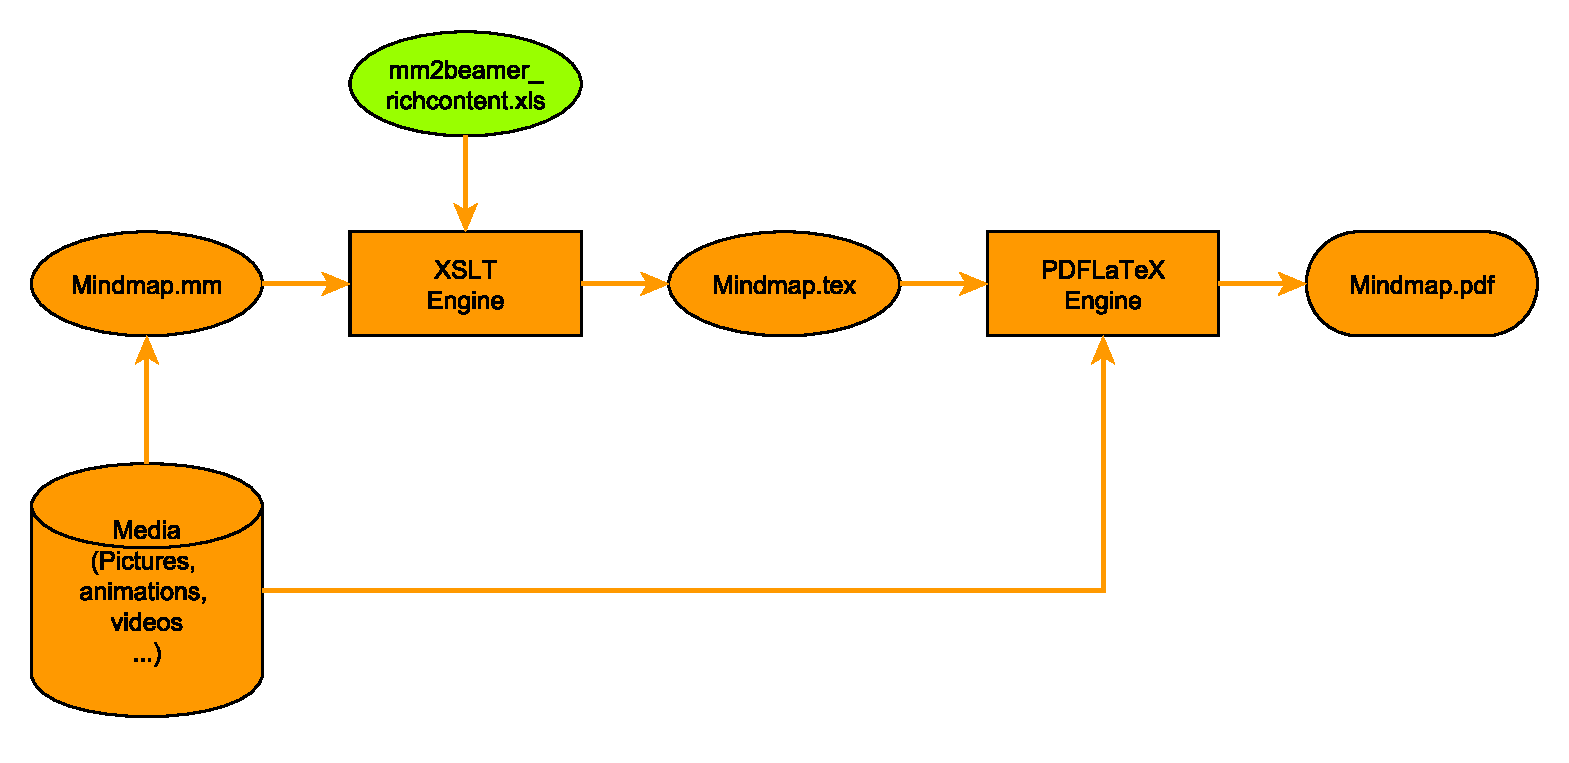
\includegraphics[width=.97\textwidth]{diagram.pdf}\newline{\scriptsize{Only works with Alt+Shift+K option. The "add image" options doe not accept pdf format. SVG files cannot be exported}}\end{figure}
\end{frame}
}



\subsection{Pause}

{
\begin{frame}\frametitle{Pause effects}
	\begin{itemize}

		\item Beamer commands such as "pause" can be used \pause
		\item Second point \pause
		\item     Third point
	\end{itemize}

\end{frame}
}






\section{Backgrounds}
		
\subsection{Background Color}

{

\beamertemplateshadingbackground{blue}{blue}
\begin{frame}\frametitle{Blue background}
	\begin{itemize}

		\item [*] This background is blue
		\begin{itemize}

			\item [] Bullets can be removed or modified by puttin "[]" at the begining of each node
		\end{itemize}
		\item [*] \color{white} This foreground is white
	\end{itemize}

\end{frame}
}





{

\beamertemplateshadingbackground{blue}{blue}
\begin{frame}[plain]\frametitle{Blue background, plain frame}
	\begin{itemize}

		\item [1] This background is blue
		\begin{itemize}

			\item [] Bullets can be removed or modified by puttin "[]" at the begining of each node
		\end{itemize}
	\end{itemize}

\end{frame}
}





{

\beamertemplateshadingbackground{red!10}{red!10}
\begin{frame}[plain]\frametitle{Custom Red background, plain frame}
	\begin{itemize}

		\item [] This background is blue
		\begin{itemize}

			\item [] Bullets can be removed by puttin "[]" at the begining of each node
		\end{itemize}
	\end{itemize}

\end{frame}
}





\subsection{Background Image}

{

\usebackgroundtemplate{\includegraphics	[width=\paperwidth,height=\paperheight]%
	{05_30_32_web.jpg}}
\begin{frame}\frametitle{Background image}
	\begin{itemize}

		\item Background images can put through the "backgroundpicture" attribute
	\end{itemize}

\end{frame}
}






\section{Frame Styles}
		
\subsection{Positioning}

{
\begin{frame}[t]\frametitle{Top}
	\begin{itemize}

		\item Text at the top of the slide
	\end{itemize}

\end{frame}
}




{
\begin{frame}\frametitle{Middle}
	\begin{itemize}

		\item Text at the middle (default)
	\end{itemize}

\end{frame}
}



{
\begin{frame}[b]\frametitle{Bottom}
	\begin{itemize}

		\item Text at the bottom
	\end{itemize}

\end{frame}
}




\subsection{Long Texts}

{
\begin{frame}[allowframebreaks]\frametitle{Allowframebreaks}
	\begin{itemize}

		\item Long texts can be adapted to slides through different options
		\item Long texts can be adapted to slides through different options
		\begin{itemize}

			\item Long texts can be adapted to slides through different options
			\item Long texts can be adapted to slides through different options
			\begin{itemize}

				\item Long texts can be adapted to slides through different options
				\item Long texts can be adapted to slides through different options
				\item Long texts can be adapted to slides through different options
				\item Long texts can be adapted to slides through different options
			\end{itemize}
		\end{itemize}
		\item Long texts can be adapted to slides through different options
		\item Long texts can be adapted to slides through different options
		\begin{itemize}

			\item Long texts can be adapted to slides through different options
			\begin{itemize}

				\item Long texts can be adapted to slides through different options
			\end{itemize}
			\item Long texts can be adapted to slides through different options
		\end{itemize}
		\item Long texts can be adapted to slides through different options
		\item Long texts can be adapted to slides through different options
		\begin{itemize}

			\item Long texts can be adapted to slides through different options
		\end{itemize}
		\item Long texts can be adapted to slides through different options
		\item Long texts can be adapted to slides through different options
		\item Long texts can be adapted to slides through different options
		\begin{itemize}

			\item Long texts can be adapted to slides through different options
			\item Long texts can be adapted to slides through different options
			\begin{itemize}

				\item Long texts can be adapted to slides through different options
				\item Long texts can be adapted to slides through different options
				\item Long texts can be adapted to slides through different options
				\item Long texts can be adapted to slides through different options
			\end{itemize}
		\end{itemize}
		\item Long texts can be adapted to slides through different options
		\item Long texts can be adapted to slides through different options
		\begin{itemize}

			\item Long texts can be adapted to slides through different options
			\begin{itemize}

				\item Long texts can be adapted to slides through different options
			\end{itemize}
			\item Long texts can be adapted to slides through different options
		\end{itemize}
	\end{itemize}

\end{frame}
}















{
\begin{frame}[shrink,plain]\frametitle{Shrink}
	\begin{itemize}

		\item Long texts can be adapted to slides through different options
		\item Long texts can be adapted to slides through different options
		\begin{itemize}

			\item Long texts can be adapted to slides through different options
			\item Long texts can be adapted to slides through different options
			\begin{itemize}

				\item Long texts can be adapted to slides through different options
				\item Long texts can be adapted to slides through different options
				\item Long texts can be adapted to slides through different options
				\item Long texts can be adapted to slides through different options
			\end{itemize}
		\end{itemize}
		\item Long texts can be adapted to slides through different options
		\item Long texts can be adapted to slides through different options
		\begin{itemize}

			\item Long texts can be adapted to slides through different options
			\begin{itemize}

				\item Long texts can be adapted to slides through different options
			\end{itemize}
			\item Long texts can be adapted to slides through different options
		\end{itemize}
		\item Long texts can be adapted to slides through different options
		\item Long texts can be adapted to slides through different options
		\begin{itemize}

			\item Long texts can be adapted to slides through different options
		\end{itemize}
		\item Long texts can be adapted to slides through different options
		\item Long texts can be adapted to slides through different options
		\item Long texts can be adapted to slides through different options
		\begin{itemize}

			\item Long texts can be adapted to slides through different options
			\item Long texts can be adapted to slides through different options
			\begin{itemize}

				\item Long texts can be adapted to slides through different options
				\item Long texts can be adapted to slides through different options
				\item Long texts can be adapted to slides through different options
				\item Long texts can be adapted to slides through different options
			\end{itemize}
		\end{itemize}
		\item Long texts can be adapted to slides through different options
		\item Long texts can be adapted to slides through different options
		\begin{itemize}

			\item Long texts can be adapted to slides through different options
			\begin{itemize}

				\item Long texts can be adapted to slides through different options
			\end{itemize}
			\item Long texts can be adapted to slides through different options
		\end{itemize}
	\end{itemize}

\end{frame}
}
















\section{Other options}
		
\subsection{Embedding videos}

{
\begin{frame}\frametitle{Animations}
	\begin{itemize}

		\item TikZ animations can be added
		\begin{itemize}

			\item They only work on Adobe Acrobat
			\item Adobe Acrobat for Linux does not support videos properly
		\end{itemize}
	\end{itemize}

\end{frame}
}



{
\begin{frame}[fragile]\frametitle{Movies}

Videos can be embedded with the "movie" latex command (from "multimedia" package): Content must be written in freeplane "notes". Not all PDF visualization programs can render it properly.

Example:
\begin{verbatim}
\movie[autostart, showcontrols, width=\textwidth,
height= 0.7\textheight , poster = false]
\includegraphics[height= 0.7\textheight]
{images/video_iconl.jpg}}{video.mov}
\end{verbatim}




\end{frame}
}




\subsection{Embedding other type of content}

{
\begin{frame}\frametitle{Other type of content}

\end{frame}
}







\end{document}